\chapter{Implementacija i korisničko sučelje}
		
		
		\section{Korištene tehnologije i alati}
			
			 {Projektni tim je tijekom izrade projekta komunicirao putem Microsoft  Teams(1) i WhatsApp(2) aplikacija. Pri izradi UML dijagrama korišten je alat Astah UML(3). Kao sustav za upravljanje izbornim kodom korišten je  Git(4), a web platforma GitLab(5) koristila se kao udaljeni repozitorij.
			 Visual Studio Code(6) koristio se kao razvojna okolina za izradu projekta. Radni okvir Express(7) u kombinaciji sa serverskim okruženjem Node.js(8) korišten je za izradu aplikacije na poslužiteljskoj strani, a na klijentskoj strani korišteni su HTML(9), CSS(9) te jezik Javascript(10). Express je brz minimalistički web radni okvir za Node.js, a značajke su mu: robusno preusmjeravnje, fokus na visoke perfomanse i http pomoćne metode. Sustav za upravljanje bazom podataka korišten na ovom projektu je PostgreSQL(11). Kao pomoć pri razmještaju korišten je Digital Ocean(12).}
		 	 
		 	 \hrule
		 	 \hfill \break
		 	 {(1) https://www.microsoft.com/
		 	 \hfill \break
		 	 (2) https://web.whatsapp.com/
		 	 \hfill \break
		 	 (3) https://astah.net/products/astah-uml/
		 	 \hfill \break
		 	 (4) https://git-scm.com/
		 	 \hfill \break
		 	 (5) https://gitlab.com/
		 	 \hfill \break
		 	 (6) https://code.visualstudio.com/
		 	 \hfill \break
		 	 (7) https://expressjs.com/
		 	 \hfill \break
		 	 (8) https://nodejs.org/en/
		 	 \hfill \break
		 	 (9) https://html.com/
		 	 \hfill \break
		 	 (10) https://www.javascript.com/
		 	 \hfill \break
		 	 (11) https://www.postgresql.org/
		 	 \hfill \break
		 	 (12) https://www.digitalocean.com/
		 	 
		 	 
		 	 
		 	 
		 	 
			
			
			\eject 
		
	
		\section{Ispitivanje programskog rješenja}
			{Svi unit testovi napravljeni su nad klasom Tank koja implementira najvažnije funkcionalnosti. Napravljeni su nad fukncijama koje izazivaju moguće poteškoće u samom kodu i tokom igranja igrice. Funkcije se odnose na koliziju tanka sa objektima na mapi. Na priloženoj slici vidimo da su svi testovi uspješno prošli.}

			\subsection{Ispitivanje komponenti}
			\begin{figure}[h]
				\centering
				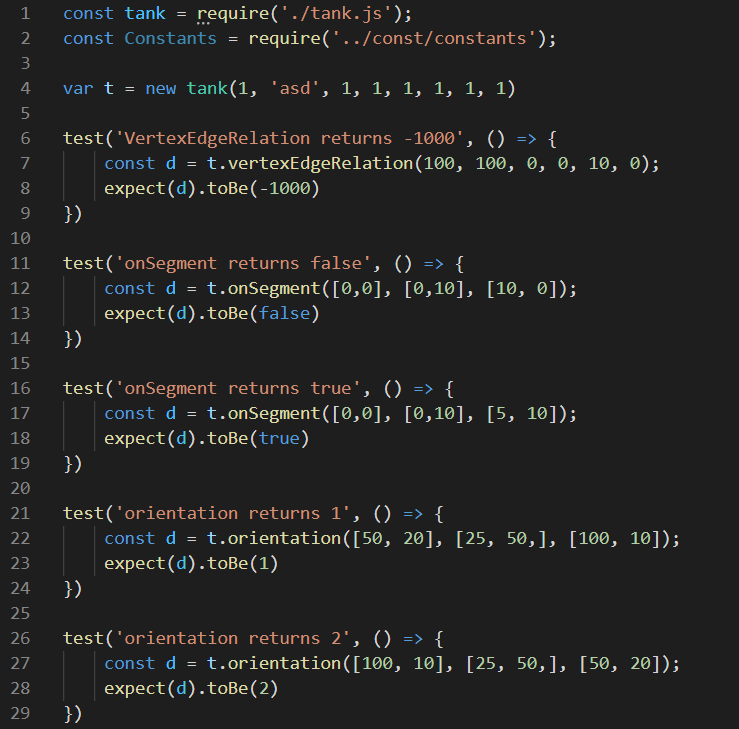
\includegraphics[width=18.5cm,height=10.5cm]{unitTests1}
				\caption{Unit testovi 1.dio}
				\label{fig:ut1}
			\end{figure}
		
			\break
			\begin{figure}[h]
				\centering
				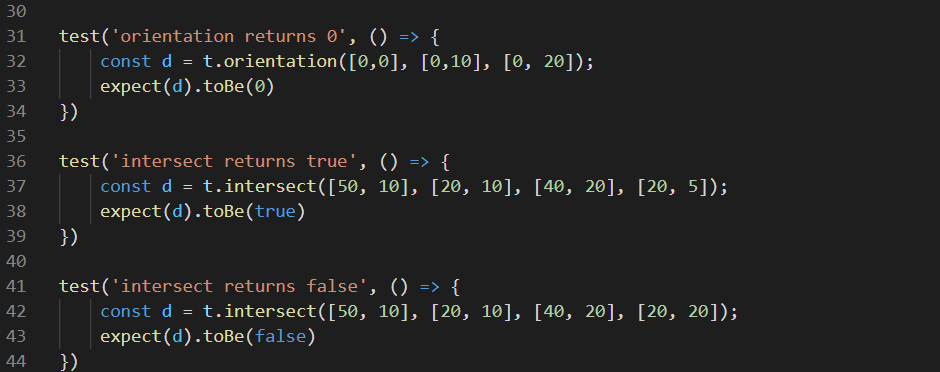
\includegraphics[width=18.5cm,height=6.5cm]{unitTest2}
				\caption{Unit testovi 2.dio}
				\label{fig:ut2}
			\end{figure}
		
		
			\begin{figure}[h]
				\centering
				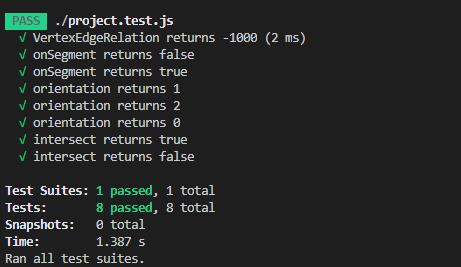
\includegraphics[width=18.5cm,height=6.5cm]{unitTestResult}
				\caption{Rezultati unit testova}
				\label{fig:ut2}
			\end{figure}
			
			
			\break
			\subsection{Ispitivanje sustava}
			
			 \textit{Potrebno je provesti i opisati ispitivanje sustava koristeći radni okvir Selenium\footnote{\url{https://www.seleniumhq.org/}}. Razraditi \textbf{minimalno 4 ispitna slučaja} u kojima će se ispitati redovni slučajevi, rubni uvjeti te poziv funkcionalnosti koja nije implementirana/izaziva pogrešku kako bi se vidjelo na koji način sustav reagira kada nešto nije u potpunosti ostvareno. Ispitni slučaj se treba sastojati od ulaza (npr. korisničko ime i lozinka), očekivanog izlaza ili rezultata, koraka ispitivanja i dobivenog izlaza ili rezultata.\\ }
			 
			 \textit{Izradu ispitnih slučajeva pomoću radnog okvira Selenium moguće je provesti pomoću jednog od sljedeća dva alata:}
			 \begin{itemize}
			 	\item \textit{dodatak za preglednik \textbf{Selenium IDE} - snimanje korisnikovih akcija radi automatskog ponavljanja ispita	}
			 	\item \textit{\textbf{Selenium WebDriver} - podrška za pisanje ispita u jezicima Java, C\#, PHP koristeći posebno programsko sučelje.}
			 \end{itemize}
		 	\textit{Detalji o korištenju alata Selenium bit će prikazani na posebnom predavanju tijekom semestra.}
			
			\eject 
		
		
		\section{Dijagram razmještaja}
		
			{Dijagram razmještaja opisuje topologiju sustava i odnos sklopovskih i programskih dijelova. Na poslužiteljskom računalu se nalaze web poslužitelj i poslužitelj baze podataka. Klijenti preko web preglednika na svom računalu pristupaju web aplikaciji. Sustav je baziran na arhitekturi ”klijent – posluzitelj”, a komunikacija između računala korisnika i poslužitelja odvija se preko HTTPS veze. Dakle, korisnik putem web preglednika šalje zahtjev web poslužitelju koji pokreće web aplikaciju i prosljeđuje joj zahtjev.}
			
			\begin{figure}[h]
				\centering
				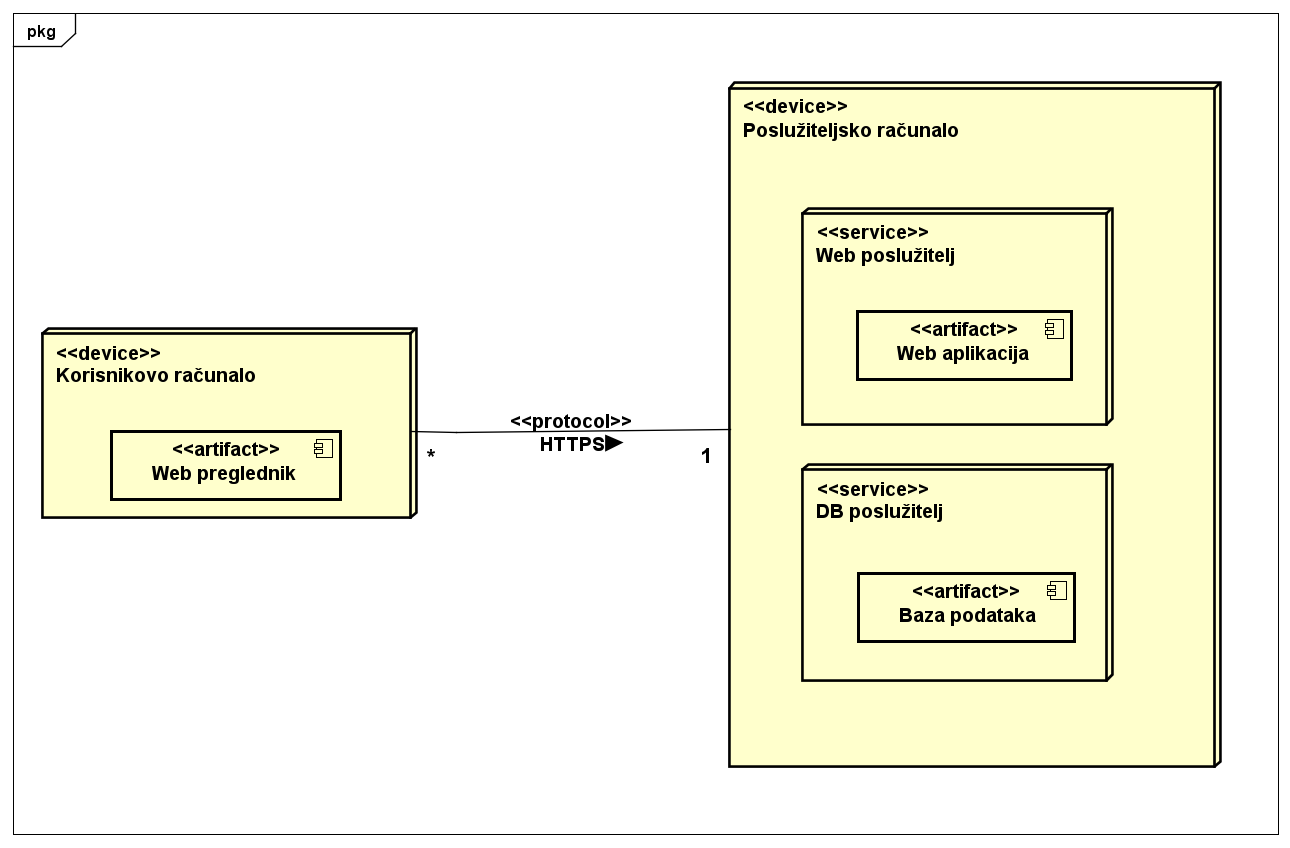
\includegraphics[width=17.5cm,height=12.5cm]{deploymentDiagram}
				\caption{Dijagram razmještaja}
				\label{fig:pkg}
			\end{figure}
			
			\eject 
		
		\section{Upute za puštanje u pogon}
		
			{Za puštanje aplikacije u pogon potreban je korisnički račun na usluzi Digital Ocean. Zapotrebe projekta, koristimo besplatnu verziju korisničkog računa. Za potrebe projekta korištena je baza podataka PostgreSQL. Konfiguracijska datoteka za bazu podataka nalazi se u datoteci izvorni\_kod/db/the\_backup.sql. Prazna baza podataka pokreće se korištenjem naredbe “psql the\_backup.sql”. Nakon toga na bazu se spaja koristeći datoteku izvorni\_kod/db/inde.js gdje se unosi korisničko ime za bazu podataka, lozinka i port. Za puštanje aplikacije u rad potrebno je klonirati repozitorij na server te pokrenuti naredbom “npm start” uz prethodno postavljanje node.js.}
			
			
			\eject 